\documentclass[11pt]{article}
\usepackage[margin=0.82in]{geometry}
\usepackage{amsmath,amssymb,bm,booktabs,array}
\usepackage{xcolor,graphicx,tikz}
\usetikzlibrary{arrows.meta,positioning}
\usepackage[most]{tcolorbox}
\usepackage{enumitem,fancyhdr,hyperref,microtype}
\definecolor{navy}{HTML}{17365D}
\definecolor{blue}{HTML}{2F75B5}
\definecolor{cyan}{HTML}{2A9D8F}
\definecolor{gold}{HTML}{E9C46A}
\definecolor{red}{HTML}{C44536}
\definecolor{lightblue}{HTML}{EAF3F8}
\hypersetup{colorlinks=true,linkcolor=navy,urlcolor=blue,citecolor=navy}
\pagestyle{fancy}\fancyhf{}
\lhead{M\&I-ENG 690A -- AI in Fluid Mechanics}\rhead{Week 7 Extension}\cfoot{\thepage}
\setlength{\headheight}{14pt}
\setlist{itemsep=3pt,topsep=4pt}
\newtcolorbox{learningbox}{colback=lightblue,colframe=blue,title=Learning checkpoint,fonttitle=\bfseries}
\newtcolorbox{warningbox}{colback=gold!18,colframe=gold!70!black,title=Important distinction,fonttitle=\bfseries}
\newtcolorbox{paperbox}{colback=cyan!6,colframe=cyan!80!black,title={Connection to Lee \& You (JFM, 2019)},fonttitle=\bfseries}
\newtcolorbox{evidencebox}{colback=white,colframe=navy,title=Evidence gate,fonttitle=\bfseries}
\newcommand{\Rey}{\mathrm{Re}}
\newcommand{\Ma}{\mathrm{Ma}}
\newcommand{\St}{\mathrm{St}}

\begin{document}
\begin{titlepage}
\centering\vspace*{1.0cm}
{\color{navy}\rule{\textwidth}{2pt}}\\[0.5cm]
{\Huge\bfseries Circular-Cylinder Wakes\\[0.18cm]with Lattice Boltzmann and Neural Prediction\par}
\vspace{0.35cm}{\Large Week 7 Extension Lecture Notes\par}
\vspace{0.5cm}{\color{navy}\rule{\textwidth}{2pt}}\\[0.9cm]
{\Large M\&I-ENG 690A -- AI in Fluid Mechanics\par}
\vspace{0.25cm}{\large Summer 2026\par}
\vfill
\begin{tcolorbox}[colback=lightblue,colframe=blue,width=0.92\textwidth]
\textbf{Central question.} Can a neural model preserve the convection, phase, strength, and shedding frequency of an unseen cylinder wake, rather than merely produce a visually smooth field?
\end{tcolorbox}
\vfill{\large Instructor: Ehsan Roohi\par}
\end{titlepage}

\tableofcontents\newpage

\section{Position in the Course}
The original course remains a six-week sequence: Weeks 1--4 establish numerical, kinetic, and surrogate-model foundations; the additive Week 4.1 develops classical POD--Galerkin and POD--DEIM for the cavity; Weeks 5--6 are the controlled research project. This cylinder module is a \emph{Week 7 extension}. It changes the geometry and the dominant physics only after the original sequence is complete.

\begin{learningbox}
By the end of Week 7, a student should be able to:
\begin{enumerate}
\item explain the physical transition from attached flow to steady recirculation and periodic vortex shedding;
\item derive the D2Q9 equilibrium distribution and BGK collision update;
\item connect $\Rey$, viscosity, relaxation time, and low-Mach restrictions;
\item measure drag, lift, recirculation length, and Strouhal number;
\item design a complete-case Reynolds holdout without snapshot leakage; and
\item diagnose phase error and downstream vortex diffusion in a learned rollout.
\end{enumerate}
\end{learningbox}

\section{Cylinder-Wake Physics}
For a cylinder of diameter $D$ in a uniform stream $U_\infty$, the governing nondimensional parameter is
\begin{equation}
\Rey_D=\frac{U_\infty D}{\nu}.
\end{equation}
At very low $\Rey_D$, the flow is attached and viscous. A symmetric recirculation bubble develops as inertia grows. The steady two-dimensional wake loses stability near $\Rey_D\approx47$, producing the alternating B\'enard--von K\'arm\'an vortex street. The precise measured transition and forces depend on blockage, domain extent, discretization, and boundary treatment.

The relevant observables are
\begin{align}
C_D &= \frac{F_D}{\tfrac12\rho U_\infty^2D}, &
C_L &= \frac{F_L}{\tfrac12\rho U_\infty^2D},\\
\St &= \frac{f_sD}{U_\infty}, &
\omega_z &= \frac{\partial v}{\partial x}-\frac{\partial u}{\partial y}.
\end{align}
Periodic lift is often the cleanest signal for estimating shedding frequency $f_s$. A credible field prediction should reproduce not only pixelwise vorticity but also the spectrum and phase of $C_L$ and the downstream decay of enstrophy.

\section{From Boltzmann Kinetics to D2Q9 LBM}
The lattice Boltzmann method evolves discrete populations $f_i(\bm{x},t)$ associated with lattice velocities $\bm{c}_i$. Density and momentum are moments:
\begin{equation}
\rho=\sum_i f_i,\qquad \rho\bm{u}=\sum_i f_i\bm{c}_i.
\end{equation}
For D2Q9,
\begin{equation}
\bm{c}_i\in\{(0,0),(\pm1,0),(0,\pm1),(\pm1,\pm1)\},
\end{equation}
with weights $w_0=4/9$, $w_{1\ldots4}=1/9$, and $w_{5\ldots8}=1/36$. The second-order isothermal equilibrium is
\begin{equation}
f_i^{eq}=w_i\rho\left[1+\frac{\bm{c}_i\cdot\bm{u}}{c_s^2}
+\frac{(\bm{c}_i\cdot\bm{u})^2}{2c_s^4}-\frac{\bm{u}\cdot\bm{u}}{2c_s^2}\right],
\qquad c_s^2=\frac13.
\end{equation}

\subsection{Collision and streaming}
The single-relaxation-time BGK update is
\begin{equation}
f_i^*(\bm{x},t)=f_i(\bm{x},t)-\frac{1}{\tau}\left[f_i(\bm{x},t)-f_i^{eq}(\bm{x},t)\right],
\end{equation}
followed by streaming,
\begin{equation}
f_i(\bm{x}+\bm{c}_i\Delta t,t+\Delta t)=f_i^*(\bm{x},t).
\end{equation}
In lattice units,
\begin{equation}
\nu=c_s^2\left(\tau-\frac12\right),\qquad
\tau=\frac12+\frac{U_\infty D}{c_s^2\Rey_D}.
\end{equation}
Thus increasing $\Rey_D$ at fixed $U_\infty$ and $D$ drives $\tau$ toward $1/2$, where numerical robustness becomes difficult. The notebook provides both transparent BGK and a more robust two-relaxation-time (TRT) option.

\begin{warningbox}
LBM is weakly compressible. Keep $\Ma=U_\infty/c_s$ small and monitor density drift. A correct nominal Reynolds number does not compensate for excessive Mach number, inadequate resolution, or boundary contamination.
\end{warningbox}

\section{Geometry and Boundary Conditions}
The computational domain must provide sufficient upstream distance, downstream wake length, and transverse clearance. The cylinder uses a circular solid mask with no-slip bounce-back. The inlet prescribes velocity; the outlet must minimize reflected disturbances; upper and lower boundaries must be consistent with the intended blockage model.

\begin{center}
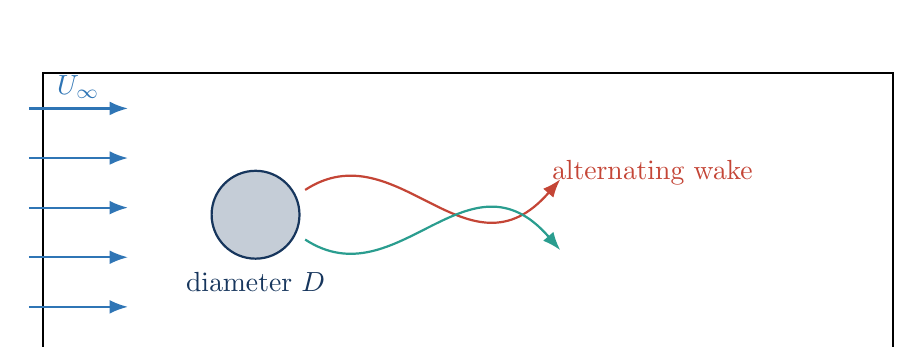
\begin{tikzpicture}[>=Latex,scale=0.9]
\draw[thick] (0,0) rectangle (12,4);
\fill[navy!25] (3,2) circle (0.62);\draw[navy,thick] (3,2) circle (0.62);
\foreach \y in {0.7,1.4,2.1,2.8,3.5}{\draw[->,blue,thick] (-0.2,\y)--(1.2,\y);}
\draw[->,red,thick] (3.7,2.35) .. controls (5,3.2) and (6,1.0) .. (7.3,2.5);
\draw[->,cyan,thick] (3.7,1.65) .. controls (5,0.8) and (6,3.0) .. (7.3,1.5);
\node[blue] at (0.5,3.8) {$U_\infty$};
\node[navy] at (3,1.05) {diameter $D$};
\node[red] at (8.6,2.6) {alternating wake};
\end{tikzpicture}
\end{center}

Halfway bounce-back is second-order accurate only for appropriately located, grid-aligned walls. A staircase representation of a circle introduces geometry error; interpolated bounce-back can reduce it. This teaching solver reports the mask and grid resolution explicitly rather than hiding this limitation.

\section{Force and Frequency Extraction}
The momentum-exchange method estimates the force transferred during population reflection. After discarding the transient, compute time-averaged drag, RMS lift, and the dominant nonzero lift-spectrum frequency. Let $t^*=tU_\infty/D$; then the frequency in $t^*$ is directly $\St$.

For a shedding case, evidence should include:
\begin{enumerate}
\item a sustained $C_L(t^*)$ oscillation after transient removal;
\item a narrow spectral peak and a stable $\St$ estimate across adjacent windows;
\item alternating signed vorticity in the wake;
\item mean $C_D$ and $\St$ compared with appropriate two-dimensional references; and
\item sensitivity to grid, domain size, time step, and sampling window.
\end{enumerate}

\begin{evidencebox}
The quick retained cases ($\Rey=5,20,40,100,180$) are teaching evidence. They demonstrate expected regimes and diagnostics, but the qualification path---not a single attractive contour---is the basis for a quantitative claim.
\end{evidencebox}

\section{Learning an Unsteady Wake}
An unsteady wake is a transport problem. Vortices translate, deform, and decay. A low-rank linear combination of global modes can smear compact structures when phase is imperfect. Pixelwise mean-square error also rewards smooth predictions, so a network can reduce loss while destroying enstrophy downstream.

\subsection{Leakage-free split}
Snapshots from one trajectory are strongly correlated. Randomly distributing them among training and test sets is leakage. The Week-7 protocol holds out an entire Reynolds-number case. Model selection uses development cases only; the unseen case is opened once after architecture and hyperparameters are frozen.

\subsection{Four-frame multi-scale CNN}
Let four consecutive input fields be
\begin{equation}
\mathcal{X}_n=[\omega_{n-3},\omega_{n-2},\omega_{n-1},\omega_n].
\end{equation}
A convolutional model predicts $\widehat{\omega}_{n+1}$. Multiple spatial scales help represent both the near-cylinder shear layers and larger downstream vortices. Recursive rollout feeds a prediction back as input, which exposes accumulated phase and amplitude error.

Useful evaluation quantities include
\begin{align}
\epsilon_{L_2}(t)&=\frac{\|\widehat{\omega}(t)-\omega(t)\|_2}{\|\omega(t)\|_2},\\
E_\omega(x_1,x_2)&=\frac12\int_{x_1}^{x_2}\int \omega^2\,dy\,dx,\\
\epsilon_{\phi}(t)&=\operatorname{wrap}\left(\widehat{\phi}(t)-\phi(t)\right).
\end{align}
Report the downstream enstrophy ratio, spectral peak, and phase error together with global $L_2$ error.

\section{Connection to the 2019 JFM Study}
\begin{paperbox}
Lee and You (2019) developed a deep-learning framework for unsteady circular-cylinder flow prediction using consecutive flow fields, convolutional processing, and recursive future prediction. Their study motivates three principles used here: temporal context must be explicit, evaluation must examine rollout rather than isolated frames, and physical diagnostics are necessary in addition to image similarity.
\end{paperbox}

The present Week-7 exercise is \emph{inspired by}, not a reproduction of, Lee and You. The domain, solver, training set, network capacity, losses, and retained resolution are deliberately smaller for transparent CPU-accessible teaching. Consequently, agreement with one animation cannot be presented as replication of the 2019 result.

The most important comparison is methodological:
\begin{center}
\begin{tabular}{p{0.24\textwidth}p{0.33\textwidth}p{0.33\textwidth}}
\toprule
Question & Lee \& You (2019) & FlowMLLab Week 7 \\
\midrule
Temporal input & Consecutive flow information & Four consecutive vorticity frames \\
Prediction test & Future-field and recursive behavior & One-step plus retained blind animation \\
Generalization & Study-specific trained/tested conditions & Complete unseen-Reynolds holdout \\
Physical assessment & Flow evolution beyond visual similarity & $L_2$, spectra, phase, divergence/no-slip, downstream enstrophy \\
Purpose & Research framework & Auditable educational extension \\
\bottomrule
\end{tabular}
\end{center}

\begin{warningbox}
A sharp first vortex followed by a diffuse downstream wake usually indicates accumulated phase/transport error, spectral damping, or an MSE-driven smoothing bias. It is not acceptable to judge the model only near the cylinder.
\end{warningbox}

\section{Notebook Workflow and Decision Gates}
The companion notebook follows this order:
\begin{enumerate}
\item derive D2Q9 equilibrium and verify moment recovery;
\item audit $\Rey$, $\Ma$, $\tau$, blockage, and boundary masks;
\item reproduce the five retained regimes;
\item examine $C_D$, $C_L$, $\St$, recirculation, and vorticity;
\item establish a POD/phase baseline and observe diffusion failure;
\item freeze the four-frame multi-scale CNN using development cases;
\item open the complete unseen-Reynolds case; and
\item report field error, spectrum, phase, divergence/no-slip, and downstream enstrophy.
\end{enumerate}

\begin{evidencebox}
Pass only if the model improves on the declared baseline without unacceptable downstream enstrophy loss or spectral/phase failure. If it fails, document the failure; do not retune on the blind case.
\end{evidencebox}

\section{Questions for Discussion}
\begin{enumerate}
\item Why can a lower global MSE coexist with a visibly worse vortex street?
\item Which error grows first in rollout: amplitude, phase, wavelength, or wake width?
\item How would a vorticity-gradient, spectral, or transport-aware loss change the bias?
\item Why is an unseen Reynolds case stronger evidence than randomly held-out snapshots?
\item Which LBM error could be learned faithfully by the CNN yet remain physically wrong?
\end{enumerate}

\section{References}
\begin{enumerate}
\item X. He and L.-S. Luo, ``Lattice Boltzmann Model for the Incompressible Navier--Stokes Equation,'' \emph{Journal of Statistical Physics}, 88, 927--944 (1997). \href{https://doi.org/10.1023/B:JOSS.0000015179.12689.e4}{doi:10.1023/B:JOSS.0000015179.12689.e4}.
\item C. P. Jackson, ``A Finite-Element Study of the Onset of Vortex Shedding in Flow Past Variously Shaped Bodies,'' \emph{Journal of Fluid Mechanics}, 182, 23--45 (1987). \href{https://doi.org/10.1017/S0022112087002234}{doi:10.1017/S0022112087002234}.
\item L. Qu, C. Norberg, L. Davidson, S.-H. Peng, and F. Wang, ``Quantitative Numerical Analysis of Flow Past a Circular Cylinder at Reynolds Number between 50 and 200,'' \emph{Journal of Fluids and Structures}, 39, 347--370 (2013). \href{https://doi.org/10.1016/j.jfluidstructs.2013.02.007}{doi:10.1016/j.jfluidstructs.2013.02.007}.
\item S. Lee and D. You, ``Data-Driven Prediction of Unsteady Flow over a Circular Cylinder Using Deep Learning,'' \emph{Journal of Fluid Mechanics}, 879, 217--254 (2019). \href{https://doi.org/10.1017/jfm.2019.700}{doi:10.1017/jfm.2019.700}.
\item M. Bouzidi, M. Firdaouss, and P. Lallemand, ``Momentum Transfer of a Boltzmann-Lattice Fluid with Boundaries,'' \emph{Physics of Fluids}, 13, 3452--3459 (2001). \href{https://doi.org/10.1063/1.1399290}{doi:10.1063/1.1399290}.
\end{enumerate}

\end{document}
